\chapter[Implementation]{Implementation} \label{ch:implementation}

\section{Introduction}
Based on the evaluation carried out in \autoref{sec:consideredtech} the \acrlong{spa} was implemented with Vue and Nuxt. To give the reader a better understanding of how the application was built, the first few sections of this chapter will discuss which additional tools and functionalities Nuxt provides, how Vue is used and how \acrfull{soc} is achieved. Later sections which describe the specific implementation of UI elements do that from a functionality-based perspective and do not go into the specifics of CSS classes used, as these are described in depth in the Bulma documentation. It is enough for the reader to have a basic understanding of CSS.

\section{Nuxt.js}
Nuxt's primary use case is to provide \acrlong{ssr} for Vue-based applications. It also advertises itself as a framework which "presets all the configuration needed to make your development of a Vue.js application enjoyable" \cite{Nuxtjs:online}. While this blurry description is not very meaningful on its own, it indicates that Nuxt pre-configures certain parts of a Vue application. The most important of which are: \acrlong{ssr}, automatic setup of routing and store management.

\subsection{Rendering modes}
Nuxt offers three rendering modes: \acrshort{ssr}, "Prerendering" and "Single Page Application". For descriptions of the first two please see \autoref{sub:seo}. The "Single Page Application" mode does not offer server-rendering capabilities while still pre-configuring routing and state management. This mode is especially useful for applications that require users to be authenticated before being able to use them. The reason why is simple: \acrlong{ssr} can only improve the SEO ranking of a page if crawlers are able to look at the full contents of it. Fully implementing \acrshort{ssr} for an application that only shows a login form would therefore be pointless. 

Then why should this project use Nuxt, which is primarily used for \acrshort{ssr} if the application cannot even profit from it because authentication prevents crawlers from seeing anything but a login form? The answer is because 1) state management and routing are auto-configured as well and 2) because in the future, the frontend might expose parts of the system in a publicly accessible way without the need of authentication. By using Nuxt from the beginning, the transition to this is much easier.

\subsection{Usage}
When using Nuxt, different folders contain different parts of the frontend application. Behind the scenes, Webpack - one of the most popular bundler tools consolidates, minifies, transforms and transpiles the code of these folders into browser-readable plain JavaScript code. 

\begin{table}
    \begin{tabularx}{\linewidth}{|l|X|}
        \hline
        \textbf{Folder} & \textbf{Description} \\
        \hline
        assets & contains un-compiled assets such as images, global css or fonts  \\
        \hline
        components & contains reusable Vue Single File Components \\
        \hline
        layouts & contains Vue files that define the applications theme \\
        \hline
        middleware & defines files which are run before a route changes, e.g check if user is authenticated before redirecting \\
        \hline
        pages & contains the pages of the application, Nuxt automatically creates routes corresponding to a page's name \\
        \hline
        plugins & contains plain JavaScript files which are run before instantiating the application, e.g used for inject adding an internationalization plugin \\
        \hline
        static & files in this is directory are directly mapped to server root and are not compiled or renamed in any way, e.g robots.txt \\
        \hline
        store & contains Vuex store files, every file added in this directory is automatically mapped to the global store \\
        \hline
        nuxt.config.js & contains the Nuxt configuration for the application, e.g which plugins and middleware to use\\
        \hline
        package.json & is not Nuxt specific but added by npm and contains application dependencies and scripts \\
        \hline
    \end{tabularx}
    \caption{Nuxt Folder Structure}
    \label{table:filestructure}
\end{table}

Typically, functional components are defined inside the components folder. These components might include other components in order to compose more complex architectures. Pages and layouts are also nothing more than Vue components, however, they are used in very specific ways. The file structure of the pages folder is automatically read by Nuxt and routes are generated from it. For example the file pages/index.vue is shown when a user visits \url{hausversammlung.at}, whereas the file pages/issues/index.vue translates to the url \url{hausversammlung.at/issues/}. Layouts are used to change the look and feel of the application. For example it is possible to create a layout file which includes a navigation bar on the top of the page. Nuxt then allows developers to set a layout property inside a page which corresponds to a layout file, resulting in easily reusable themes. 

\section{Vue}
This section aims to extend the basic description of Vue's usage as described in \autoref{subsub:vueusage} so that code samples of this chapter are more easily understood. For the sake of brevity, some parts will be omitted if they are not crucially relevent (e.g transitions). 

\subsection{Separation of Concerns}
A very important aspect of modern software architectures is \acrfull{soc} which is often regarded to as principles of modularization of code and object-oriented design \cite{laplante2007every:book}. In the case of traditional web design HTML, CSS and JavaScript are often physically separated (separation of file types) leading to increased maintainability of code, a less tightly coupled system and decreased probability of violating DRY principles. Furthermore, it helps building complex layered systems which can be actively worked on by multiple developers. 

Vue however, takes different approaches on \acrshort{soc} depending on the way it is used in a project:
either Vue.js is added to existing sites by using a standard HTML script tag or by using a complete bundling tool like Webpack or Browserify to add it as a dependency. Using Vue by adding a script tag has some disadvantages: it only allows developers to target a specific HTML container element on the page Vue is embedded in, and also brings certain disadvantages such as no CSS support inside the Vue component itself and no build steps which requires the developer to fall back to plain HTML and ES5 JavaScript rather than using various preprocessors. \newline

\begin{lstlisting}[caption=Vue component without bundler, captionpos=b, style=htmlcssjs]{Vue component without bundler}
Vue.component('todo-component', {
    template: '<h1> {{ newItem }} </h1>',
    data() {
        return {
            items: [
                {
                    id: '1',
                    title: 'Buy milk',
                    completed: false
                },
            ],
            newItem: ''
        };
    },
    methods: {
        addItem() {
            // LOGIC OMITTED FOR READABILITY
        }
\end{lstlisting}
The more preferable approach would be to use a so called “Single File Component”, a file with a “.vue” extension. These files however have to be compiled with build tools like Webpack or Browserify to extract the corresponding concerns. A sample file is depicted in \autoref{lst:sfc}. \newline

\begin{lstlisting}[caption=Vue Single File Component, label={lst:sfc}, captionpos=b, style=htmlcssjs]{Vue Single File Component}
<template>
  //HTML
  <p>{{ text }}</p>
</template>

<script>
//JS
export default {
  data() {
    return {
      text: 'Hello World!'
    }
  }
}
</script>

<style scoped>
//CSS
  p {
    color: red;
  }
</style>
\end{lstlisting}

By defining .vue files developers can utilize syntax highlighting, linting and component-scoped CSS. Furthermore preprocessors like Pug, Babel or SASS can be used to further improve the development process. This however comes with an important tradeoff: as Single File Components rely on the use of build tools, they are not very suitable projects which are not completely vue-based

Clearly HTML, CSS and JavaScript are not separated into their own respective files even when using Single File Components which leaves us with the question of how Separation of Concerns is achieved. As stated in the Vue Documentation: 

\begin{quotation}
“... separation of concerns is not equal to separation of file types. In modern UI development, we have found that instead of dividing the codebase into three huge layers that interweave with one another, it makes much more sense to divide them into loosely-coupled components and compose them. Inside a component, its template, logic and styles are inherently coupled, and collocating them actually makes the component more cohesive and maintainable \cite{VueSeparationofConcerns:online}.” 
\end{quotation}

Instead of creating different files in which logic, presentation and design are separated, Vue consolidates these parts into a single file, hence the name “Single File Component”, making the code more maintainable and comprehensible. It is important to note that throughout the project, Single File Components are used. 

\subsection{Interpolation}
Interpolation in Vue is the process of substituting a "placeholder" inside HTML with a real value. This special syntax is also referred to as "Mustache" syntax. \autoref{interpolation} depicts a simple example in which the mustache "msg" tag will be replaced with the corresponding property of the component's data object. Furthermore, when the value changes, Vue automatically takes care of updating the rendered element. \newline

\begin{lstlisting}[caption=Interpolation Example, captionpos=b, style=htmlcssjs, label=interpolation]{Vue Interpolation Example}
  <span> Noticeboard-Message: {{ msg }} </span> 
\end{lstlisting}

\subsection{v-bind}
Due to technical restrictions the mustache syntax cannot be used for HTML attributes. Instead a so called "Vue directive" is utilized. Directives are way of telling Vue that a function should be applied to a specific DOM element. In the case of "v-bind" it is to bind data (value) to an attribute (key). \newline

\begin{lstlisting}[caption=v-bind Example, captionpos=b, style=htmlcssjs, label=vbind]{v-bind Example}
  //long
  <a v-bind:href="url">dynamic link</a>
  //shorthand
  <a :href="url">dynamic link</a>
\end{lstlisting}

Common examples are href attributes or dynamically bound css classes. Usually, instead of writing "v-bind:" it's shorthand is used which is just a single colon. It is important to note that this type of interpolation only works in a unidirectional way from the data object of a component to its placeholder. 

\subsection{v-model}
For elements where user input is crucial, the "v-model" directive is used. It allows for user input to change the data object's properties. In Vue terms this is referred to as "two-way data binding". \autoref{vmodel} depicts an example use case: a user inputs data into an input field, whatever they type will be displayed below it. \newline

\begin{lstlisting}[caption=v-model Example, captionpos=b, style=htmlcssjs, label=vmodel]{v-model Example}
  <input v-model="message">
  <p>Message of user: {{ message }}</p>
\end{lstlisting}

Behind the scenes, this directive uses a combination of v-bind and input events to provide this type of functionality. In reality it is only syntax sugar. This also means that while v-model works for input, textarea and select elements by default it can be implemented for custom input elements as well by utilizing v-bind and events.

\subsection{v-on}
The directive "v-on" is used in order to catch events that are emitted by a component. \newline

\begin{lstlisting}[caption=v-on Example, captionpos=b, style=htmlcssjs, label=vmodel]{v-on Example}
  //long
  <PollItem v-on:click="alert('component clicked')">
  //shorthand
  <PollItem @click="alert('component clicked')">
\end{lstlisting}

In this case, whenever the "click" event is emitted inside the PollItem component it is caught and an alert is displayed. Similarly to "v-bind", "v-on" also offers a shorthand syntax with the "@" symbol. 

\subsection{v-for}
To display multiple items at once, the directive "v-for" can be used. It counts the number of elements of a given object and iterates over each to render some defined output. \newline

\begin{lstlisting}[caption=v-for Example, captionpos=b, style=htmlcssjs, label=vmodel]{v-for Example}
  <ul>
    <li v-for="item in items">
      {{ item.message }}
    </li>
  </ul>
\end{lstlisting}

\subsection{v-if}
To conditionally show or hide elements the directive "v-if" can be used. It not only simply hides an element when its "v-if" condition resolves to a falsy value, it completely removes it from the DOM. This means from an end-user perspective it is not possible to access this element, not even by looking at the raw HTML. \newline

\begin{lstlisting}[caption=v-if Example, captionpos=b, style=htmlcssjs, label=vmodel]{v-if Example}
  <NoticeboardItem v-if="showItem">
\end{lstlisting}

The very similar directive "v-show" uses additional CSS to conditionally hide elements, without removing them from the DOM - which is a cheaper operation. This can drastically improve performance in case there are very large nested elements which often switch between hidden or shown.

\subsection{props}
Props are a way of passing data from a parent component into a child component. Addtionally, rules can be set up to validate a prop's value before it is used. \autoref{props} shows how a message prop of type String is defined inside a component. \newline

\begin{lstlisting}[caption=Props Example, captionpos=b, style=htmlcssjs, label=props]{Props Example}
  <template>
    <div>
    {{ message }}
    </div>
  </template>

  <script>
  export default {
    props: {
      message: {
        type: String,
        required: false,
        default: ""
      }
    }
  };
  </script>
\end{lstlisting}

\subsection{Component Communication}
GUI based applications typically rely on event-driven programming paradigms. Vue is no exception: events are emitted and caught and dictate the course of actions of the application. Typically, props are used to pass data from a parent to a child component, whereas events are emitted with a paylod from a child and are caught in the parent with the "v-on" directive. For heavily nested components however, a so called "event bus" or the vuex store is used which makes data available directly where it is needed instead of having to pass it from the deepest child to the highest parent. This project makes use of the props/events method and the vuex store.

\subsection{Vuex}
Vuex is a supporting library for Vue based on the Flux architecture to provide a solution for shared state management. Its concept revolves around a global state which is retrieved with "getters" and altered with "mutations" which in turn are commited by "actions". Mutations change the state's data synchronously so every change is trackable with debugging tools. Actions can be asynchronous and are often used for retrieving data from an API and then updating the system's state by passing this data to a mutation and commiting it. The term used for executing an action is "dispatch". It is important to note that while it is perfectly sensible to create methods in Vue components that reach out to an API and then commit a mutation, it makes far more sense to move these methods to the store as actions, especially if they are reused across the application. Vuex uses a "single state tree" - one JavaScript object that contains the entirety of the application's state. The state is either retrieved directly and unchanged or through getters which provide a way of transforming the returned data first. For example it is possible to directly retrieve the authentication token from the state and manually check its validity or by defining a getter which returns the users authentication state as a boolean value which depends on the token. Additionally, the store can be split up into "modules" and is done so in this project: a store file corresponds to a group of actions, getters and parts of the state. This greatly improves maintainability of the project by making it more comprehensible. \autoref{vuexsamples} illustrates some commonly used ways of interacting with the store. \newline

\begin{lstlisting}[caption=Vuex Usage, captionpos=b, style=htmlcssjs, label=vuexsamples]{Vuex Usage}
  ...mapGetters("auth", ["isAuthenticated"])
  this.$store.getters["auth/isAuthenticated"]
  ...mapState("auth", ["token", "id"])
  this.$store.state.auth.token
  ...mapActions("issues", ["getIssues"])
  this.$store.dispatch("issues/getIsses")
\end{lstlisting}


% Discusses:
% Single File Components separated into HTML, JS and CSS
% v-bind and shorthand, v-model
% ternary expressions
% events how they are emitted and caught
% props
% methods
% computed properties
% v-if 
% conditional classes 
% vuex store
% routing
% axios

\section{Authentication}
In order to use the application, users have to be authenticated. They must provide an email address and a password to a login form and request authentication. \autoref{usecase:login} depicts the detailed flow for this use case. The API then checks if the user can be authenticated and if successful issues a token, refresh token and their respective expiry times. To improve the system's usability, this data is then persisted by using cookies (see \autoref{persauthdata}). Everytime a user wants to move to a different subpage, the validity in terms of expiry time of the tokens is checked. Nuxt lets developers define "middleware" - code which is run before any page change. The middleware which is depicted in \autoref{authmiddleware} checks for one of three scenarios:

\begin{enumerate}
  \item User is authenticated \& both tokens too old -> logout
  \item User is authenticated \& only refresh token is valid -> tokens can be refreshed
  \item User is not authenticated -> read from cookies
\end{enumerate}

* A user is authenticated if the tokens and expiry times exist in \textbf{state}, they do not necessarily have to be valid (this is checked by the middleware) 

In scenario 1, there is nothing the application can do to retrieve a new set of tokens, the user manually has to request authentication again. They are therefore logged out of the system, which happens by clearing every cookie file and every property of the state. This is important because if a different user would try to log into the system but the data is not cleared first, they might encounter some information of the previous user such as Noticeboard or Poll entries which are cached in state. In scenario 2 the token has expired but the refresh token is still valid, which means the application can automatically request a refresh. In scenario 3 a user is not authenticated at all. The application therefore tries to retrieve data from cookies if they exist. This is mainly done for usability as the state is nothing more than an in-memory JavaScript object and is cleared whenever a user exits the browser or manually refreshes the page, meaning the user would have to login over and over again. When a user interacts with the application and therefore the API, they may encounter a "401 unauthorized" error which means that the user does not have valid authentication details. Axios which is used to interact with the API is extendend with a custom defined plugin that instructs it to catch these types of errors and to immediately log out the user. \autoref{unauthorized} shows how this is implemented.

\subsection{Authorization}
Not only do users have to be authenticated, they also have to be authorized for specific requests. From the API's perspective there are three access levels (the lower the number the higher the authorization level): 

\begin{itemize}
  \item Proprietor - Access Level 1
  \item Facility Management - Access Level 2
  \item Tenant - Access Level 3
\end{itemize}

What a user can do is dependant on their access level and is illustrated in the use case diagram depicted in \autoref{fig:sytemdesign}.
Because a user can be assigned to several houses and can have a different role in each one the roles are not contained inside the user object, but appended as a property for each house.

\subsection{Summary}
Users are authenticated by sending email and password to the API which in turn issues token, refresh token and expiry times. This data is persisted with cookies to improve usability. Before any page change the authentication state of the user is checked with middleware. When a request returns a "401 unauthorized" error this is caught by Axios and the user is logged out. Users can have one of three roles for every house they are assigned to, these roles dictate what a user is and is not allowed to do.

\section{Common UI Items}
In \autoref{sec:uisummary} common UI elements were identified. These include: a Navigation Bar and Search Bar. Additionally, there are various forms for creating different entries. What every form needs is a way of saving the content or cancelling the creation process - a reusable button set which provides functionality for saving and cancelling is sensible. This section discusses how these UI elements are implemented.

\subsection{Navigation Bar}
The navigation bar is used to provide quick-access links to various site-destinations of the application.
As the application uses Bulma as the underlying CSS framework, all UI items have to adhere to its guidelines for styling elements. The specific classes needed to build a Navigation Bar are depicted in \autoref{fig:navbardoc}. 

\begin{figure}[H]
  \begin{center}
  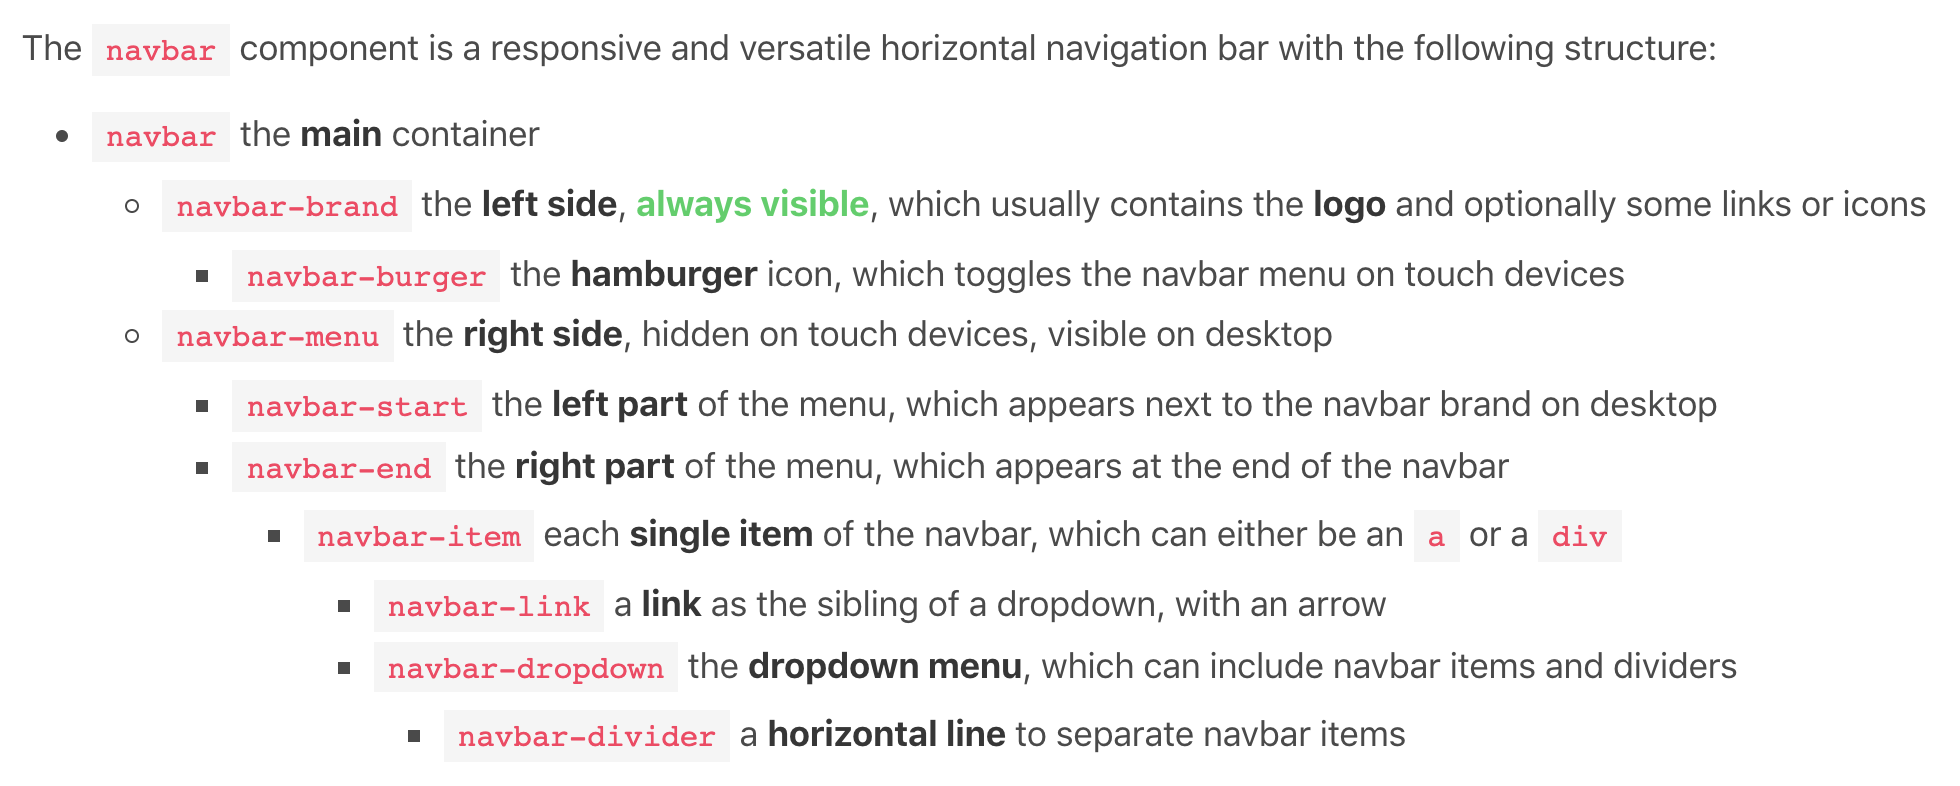
\includegraphics[width=\linewidth]{navbar-doc}
  \end{center}
  \caption{Navbar Documentation}
  \label{fig:navbardoc}
\end{figure}


The Navbar is a special component: it seems like it is reused across all pages but in reality it is only defined once in the global layout file. In Vue, it is a common convention to such components with "The" in the file name. For example the navigation bar is defined in a file called "TheNavbar.vue". When a component is used only once, it would theoretically be possible to hardcode links and other objects into that component, without decreasing maintainability However, it makes for much cleaner code to outsource these into a parent component and pass them as props. For example the navigation bar defines a prop of type array which is used to pass all links that should be displayed. In the template section the "v-for" directive is then used to iterate over each link and to render it. Depending on the user's access levels, some links are hidden. For example the "Polls" link is hidden for user roles that are not of type proprietor. Additionaly, props are used in order to set the color and dropwdown shadow of the navbar.

Dynamic classes are used to make the hamburger menu (mobile) or dropdown menu (desktop) of the navbar interactive. When a user clicks on it, the click event is caught and the data properties "burgerActive" and "dropdownActive" are set to true. Vue recognizes this change and dynamically adds the "is-active" class to the respective HTML tags which results in the right dropdown menu to expand or the hamburger menu transform into an "X" like shape. \autoref{fig:navbar} illustrates the finished component when rendered.

\begin{figure}[H]
  \begin{center}
  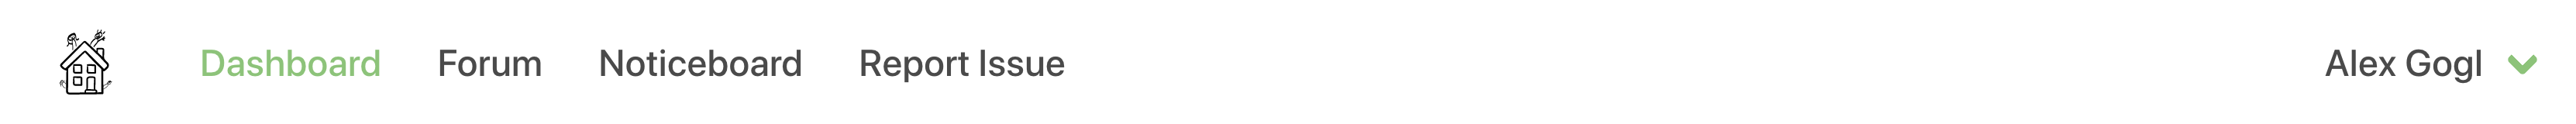
\includegraphics[width=\linewidth]{navbar}
  \end{center}
  \caption{Navbar}
  \label{fig:navbar}
\end{figure}


\subsection{Search Bar \& Create Button}
The search bar and the create button can easily be 

\subsection{Navigation Bar}

\section{Noticeboard}

\autoref{sub:noticeboardui}
\section{Forum}

\section{Polls}

\section{Issue Log System}

\section{Internationalization}
